% Created 2022-03-02 Wed 08:45
% Intended LaTeX compiler: pdflatex
\documentclass[11pt]{article}
\usepackage[utf8]{inputenc}
\usepackage[T1]{fontenc}
\usepackage{graphicx}
\usepackage{grffile}
\usepackage{longtable}
\usepackage{wrapfig}
\usepackage{rotating}
\usepackage[normalem]{ulem}
\usepackage{amsmath}
\usepackage{textcomp}
\usepackage{amssymb}
\usepackage{capt-of}
\usepackage{hyperref}
\usepackage{braket}
\usepackage{relsize}
\usepackage{amsmath}
\newcommand{\kp}{\ket{\psi}}
\newcommand{\bp}{\bra{\psi}}
\newcommand{\tr}[1]{\textrm{tr}\left[{#1}\right]}
\newcommand{\U}{\mathcal{U}}
\author{Frank Lu}
\date{\today}
\title{}
\hypersetup{
 pdfauthor={Frank Lu},
 pdftitle={},
 pdfkeywords={},
 pdfsubject={},
 pdfcreator={Emacs 27.1 (Org mode 9.5)}, 
 pdflang={English}}
\begin{document}

\tableofcontents

% Theoretical results section
\newcommand{\nH}{n_H}
\newcommand{\nV}{n_V}
\newcommand{\NH}{N_H}
\newcommand{\NV}{N_V}

\newcommand{\ls}{l_1l_2 \dots l_{\nH}}
\newcommand{\ones}{1, 1, \dots, 1}
\newcommand{\ks}{k_1k_2 \dots k_{\nH}}

\newsavebox{\mybox}
\newenvironment{Notes}
{\begin{lrbox}{\mybox}\begin{minipage}{\textwidth}}
{\end{minipage}\end{lrbox}\fbox{\usebox{\mybox}}\\}

\section{Notation}
\label{sec:orgcdf4280}
Firstly, define \(N_H\) and \(N_V\) to be the number of hidden and visible units respectively.
\(H_h\) is a vector of weights for the hidden units, where \(h = 1, 2, \dots, N_H\).
Similarly, \(V_v\) is a vector of weights for the visible units, where \(v = 1, 2, \dots, N_V\).
\(W_{h v}\) is a matrix of weights. \(C^{(hv)}_{kl}\) is the coupling matrix between the \(h\)th hidden unit and the \(v\)th visible unit. For simplicity, we will assume that \(C\) is a \(d \times d \) matrix.

\subsubsection{Note on the coordination number}
\label{sec:org17d4821}
\(n^{(h)}_V\) is the coordination number for visible units of the  \(h^{\text{th}}\) hidden unit. This is the number of connected visible units. Similarly, \(n^{(v)}_H\) is the coordination number for hidden units of the  \(v^{\text{th}}\) visible unit.

Throughout this section, we are operating on the last visible unit (the \({\NV}^{\text{th}}\) unit), which is connected to \(\nH^{(\NV)}\) hidden units. Since it is clear which visible unit we are referring to, the superscript will be omitted.

In the general case, \(\nH = \NH\) as the hidden and visible units form a complete bipartite graph. In the Snake RBM case, each visible unit is connected to exactly one hidden unit so \(\nH = 1\).

\begin{center}
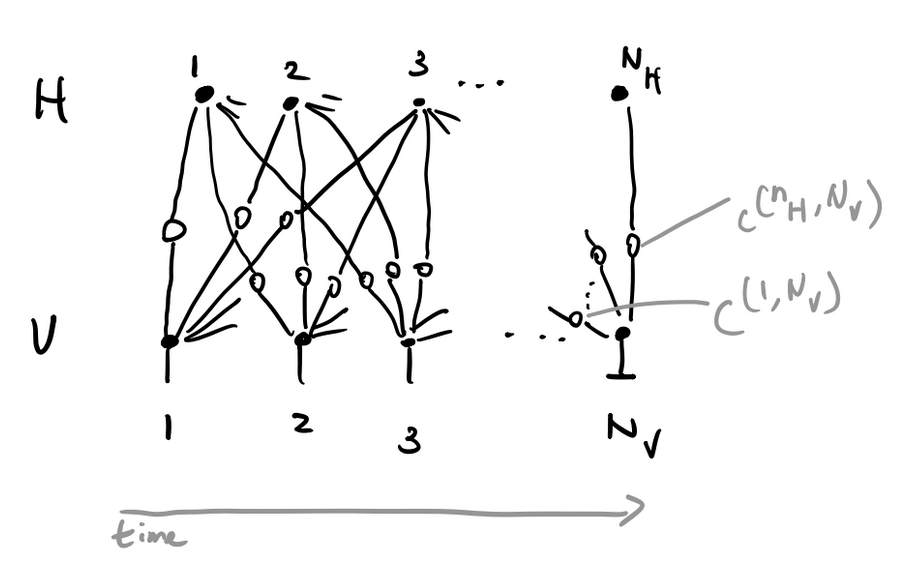
\includegraphics[scale=0.3]{/home/frank/shared/quantum/honours-thesis/theoretical-results/theoretical-results.org_20220301_152814_TaDhUt.png}
\end{center}


\section{Imposing the causality condition on RBMs}
\label{sec:orgc668679}

\begin{center}
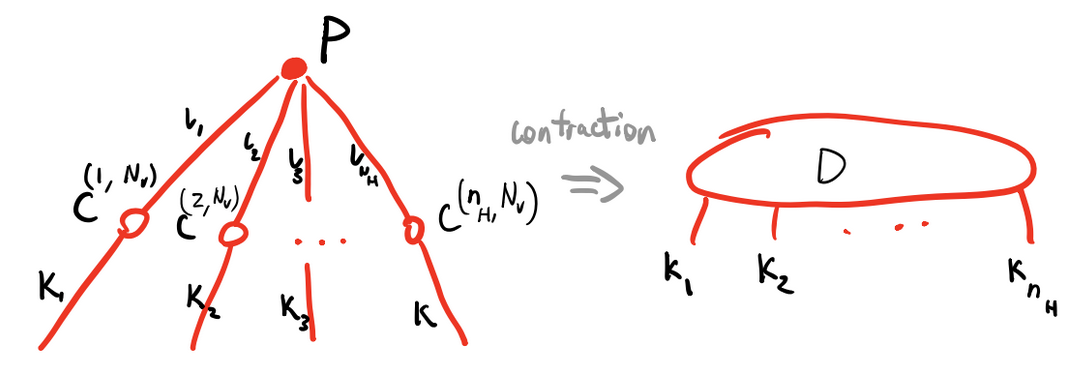
\includegraphics[scale=0.3]{/home/frank/shared/quantum/honours-thesis/theoretical-results/theoretical-results.org_20220301_153031_ZzL8yB.png}
\end{center}

Let \(D_{\ks}\) be the contraction of the red network, and \(\ket{+}\) to be a vector of \(1\)s.


If the causality condition were to hold, then,
\begin{equation} \label{eqn}
    D = \underset{\nH}{\bigotimes} \ket{+}.
\end{equation}

This is represented visually as
\begin{center}
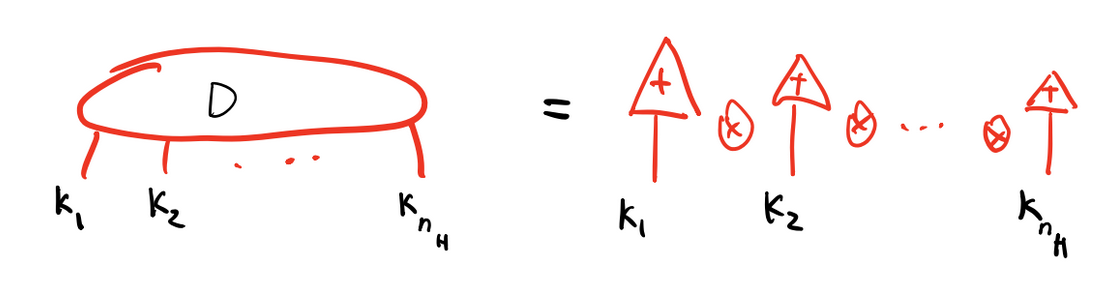
\includegraphics[scale=0.3]{/home/frank/shared/quantum/honours-thesis/theoretical-results/theoretical-results.org_20220301_153048_iHC4Hl.png}
\end{center}

The RHS is then a tensor of \(1\)s. This amounts to an a set of equations where each element of \(D\) must equal \(1\).

\subsection{Preliminary steps}
\label{sec:org49b2dc3}
Let \(P\) be the contraction of the vectorised identity with the copy tensor, and let \(k = \sqrt{d}\).
The index at which a one appears in the vectorised identity is given by a sequence \(S = (s_1, s_2, \dots, s_k )\) where \(s_i = k(i - 1) + i\) for \(1 \leq i \leq k\).


\[
P_{\ls} = \begin{cases}
  1 & l_1 = l_2 = \dots = l_{\nH} \text{ and } l_1 \in S \\
  0 & \text{otherwise}
\end{cases}
\]

\subsection{Defining the coupling matrices}
\label{sec:orgd833376}
% Note: More details of the original equation in quantum_notes.

\(C^{(hv)}_{kl}\) is a \(d \times d\) coupling matrix between the \(h\)th hidden and \(v\)th visible unit.

In our notation, we extend \(k\) and \(l\) to range over \([1, d] \), so a more useful definition could be as follows.

\begin{equation}
C^{(hv)}_{k l} = e^{{W}_{h,v} (k - 1) (l - 1) + \frac{{H}_{h} (k - 1)}{N_H} + \frac{{V}_{v} (l - 1)}{N_V}}
\end{equation}


\subsection{Equation for elements of the contracted tensor}
\label{sec:org32ad07f}

In fact, we can solve for specific elements of the \(D\) tensor.

\begin{align}
D_{\ks} &= \sum_{\ls} P_{\ls} C^{(1,\NV)}_{k_1 l_1} C^{(2,\NV)}_{k_2 l_2} \cdots C^{(\nH,\NV)}_{k_{\nH} l_{\nH}} \\
  &= \sum_{s \in S} P_{ss \dots s} C^{(1,\NV)}_{k_1 s} C^{(2,\NV)}_{k_2 s} \cdots C^{(\nH,\NV)}_{k_{\nH} s} \\
  &= \sum_{s \in S} C^{(1,\NV)}_{k_1 s} C^{(2,\NV)}_{k_2 s} \cdots C^{(\nH,\NV)}_{k_{\nH} s} \\
  &= \sum_{s \in S} \prod_{h=1}^{\nH} C^{(h,\NV)}_{k_h, s} \label{d_tensor_matrix_elem} \\
  &= \sum_{s \in S} \prod_{h=1}^{\nH} e^{{W}_{h,N_{V}} ({k}_{h} - 1 )(s - 1) + \frac{{V}_{N_{V}} (s - 1)}{N_{V}}  + \frac{{H}_{h} ({k}_{h} - 1)}{N_{H}}} \label{d_tensor_elem}
\end{align}

\subsubsection{A special case with no solutions}
\label{sec:orgf5dd7e0}
Using the general equation \eqref{d_tensor_elem}, we can solve for the very first element of the tensor, \(D_{\ones}\). (Here, let \(k_1 = k_2 = \dots = k_{\nH} = 1\).)

\begin{align}
 D_{\ones} &= \sum_{s \in S} \prod_{h=1}^{\nH} e^{ (s -1) \frac{V_{\NV}}{\NV} } \\
    &= \sum_{s \in S} e^{ (s -1) \frac{\nH V_{\NV}}{\NV} } \label{d_tensor_first_elem}
\end{align}

Suppose that \(d = 4\) (the case that \(C^{(hv)}\) is a \(2 \times 2\) matrix), then \(S = (1, 4)\).

\begin{align}
D_{\ones} &= \sum_{s \in \{1, 4\}} e^{ (s -1) \frac{\nH V_{\NV}}{\NV} } \\
    &= e^{0} + e^{ \frac{3 \nH V_{\NV}}{\NV} }
\end{align}

But requiring \(D_{\ones} = 1\) implies \(\exp(\frac{3 \nH V_{\NV}}{\NV}) = 0\), which has no solution.

In fact, the number of terms in the summation in \eqref{d_tensor_elem} is equal to the length of \(S = \sqrt{d}\).

\subsection{Interpreting results for Uniform RBMs}
\label{sec:org8955aa1}
Up until now, we have been considering the general case of fully-connected RBMs.
Consider the special subset of RBMs where all coupling matrices are identical. That is, for all \( 1 \leq h_1, h_2 \leq \nH\), and \(1 \leq v_1, v_2 \leq \NV \),

\begin{equation}
C^{(h_1 v_1)}_{kl}  = C^{(h_2 v_2)}_{kl}
\end{equation}

It immediately follows from the definition of the coupling matrices, that all entries of \(W\), \(H\), and \(V\) are also identical.
So the subscripts for the indices can be ommitted. This means that \eqref{d_tensor_matrix_elem} can be simplified.

\begin{align}
D_{\ks} &= \sum_{s \in S} \prod_{h=1}^{\nH} C^{(h,\NV)}_{k_h, s} \tag{\ref{d_tensor_matrix_elem} revisited} \\
  &= \sum_{s \in S} \prod_{h=1}^{\nH} e^{{W} ({k}_{h} - 1 )(s - 1) + \frac{{V} (s - 1)}{N_{V}}  + \frac{{H} ({k}_{h} - 1)}{N_{H}}}
\end{align}


\subsection{Interpreting results for  minimally-connected RBMs}
\label{sec:orgedc0d18}
Consider a subset of RBMs that are connected in a minimal way\ldots{}

We will call this the \emph{Snake RBM}.

``Snake RBM'' has this form.

\begin{center}
\includegraphics[scale=0.2]{/home/frank/shared/quantum/project/quantum_notes.org_20220219_132339_Pqa5Ov.png}
\end{center}


Solving the Snake RBM amounts to solving the following simplified equation.

\begin{center}
\includegraphics[scale=0.2]{/home/frank/shared/quantum/project/quantum_notes.org_20220219_132241_ktwlgT.png}
\end{center}
\end{document}
